%versi 3 (22-07-2020)
\chapter{Perancangan}
\label{chap:perancangan}
Bagian ini akan menjelaskan mengenai perancangan yang digunakan dalam membangun perangkat lunak. 


\section{Perancangan Tabel Data Wilayah}
\label{sec:perancanganTabelDataWilayah}
Pada tabel data wilayah merupakan entitas utama dalam pengembangan perangkat lunak. Perancangan tabel data wilayah dapat dilihat dari tabel \ref{tab:tabelDataWilayah}.
\begin{table}[H]
	\centering
	\caption{Rancangan Tabel Data Willayah}
	\label{tab:tabelDataWilayah}
	\resizebox{\columnwidth}{!}{%
		\begin{tabular}{|l|l|c|c|c|c|c|c|}
			\hline
			\multicolumn{1}{|c|}{\textbf{No}} &
			\multicolumn{1}{c|}{\textbf{Atribut}} &
			\textbf{Tipe} &
			\textbf{Ukuran} &
			\textbf{Primary Key} &
			\textbf{Foreign Key} &
			\textbf{Null} &
			\textbf{Keterangan} \\ \hline
			1 & id                         & Integer & 11 & Yes & - & No & AUTO\_INCREMENT \\ \hline
			2 & nama\_kelurahan            & Varchar & 80 & -   & - & No & -               \\ \hline
			3 & luas\_kelurahan            & Float   & -  & -   & - & No & -               \\ \hline
			4 & luas\_kelurahan\_prediksi  & Float   & -  & -   & - & No & -               \\ \hline
			5 & luas\_rth\_kelurahan       & Float   & -  & -   & - & No & -               \\ \hline
			6 & persentase\_rth\_kelurahan & Float   & -  & -   & - & No & -               \\ \hline
			7 & link\_googlemapss          & Varchar & -  & -   & - & No & -               \\ \hline
		\end{tabular}%
	}
\end{table}


\section{Perancangan Kelas Controller}
\label{sec:perancanganController}
\begin{enumerate}
	\item \textit{function home}
	\begin{itemize}
		\item Masukan : -
		\item Keluaran: \textit{view} homePage
		\item Tabel yang diakses: data\_wilayah
		\item Deskripsi: Menampilkan halaman utama
		\item Algoritma: -
	\end{itemize}
\end{enumerate}

\section{Perancangan Fungsi}
\label{sec:javascript}

Perancangan fungsi pada perangkat lunak berguna untuk pengembangan agar lebih dinamis dan iteraktif. Dalam perancangan perangkat lunak akan terdapat \textit{script} yang digunakan untuk pembuatan dropdown dan penggunaan radio dalam menampilkan gambar area hijau kelurahan. 

Fungsi \textit{JavaScript} \ref{code:jsdropdown} menggunakan jQuery untuk mengatur perilaku halaman web berdasarkan pilihan pengguna pada dropdown. Ketika pengguna memilih nilai pada dropdown, elemen-elemen tertentu akan disembunyikan atau ditampilkan berdasarkan nilai yang dipilih. Fungsi ini memungkinkan untuk menyesuaikan tampilan halaman secara dinamis sesuai dengan pilihan pengguna dan meningkatkan pengalaman pengguna dalam menggunakan website.

\begin{lstlisting}[language=JavaScript, caption=Fungsi Dropdown,label={code:jsdropdown}]
	$(document).ready(function() {
		$(".box").hide();
		$(".box2").hide();
		
		$(".dropdown1").change(function() {
			var optionValue = $(this).val();
			if (optionValue) {
				$(".box").not("." + optionValue).hide();
				$("." + optionValue).show();
			} else {
				$(".box").hide();
			}
		});
		
		$(".dropdown2").change(function() {
			var optionValue = $(this).val();
			if (optionValue) {
				$(".box2").not("." + optionValue).hide();
				$("." + optionValue).show();
			} else {
				$(".box2").hide();
			}
		});
	})

 
\end{lstlisting}

Fungsi \textit{JavaScript} \ref{code:jsradio} menggunakan jQuery yang memberikan fungsionalitas interaktif pada halaman web dalam mengontrol tampilan gambar berdasarkan pilihan radio yang dipilih oleh pengguna. Fungsi dapat menggunakan \textit{event handler change} pada input radio. Oleh karena itu, pengguna dapat secara dinamis mengubah gambar yang ditampilkan sesuai dengan pilihan dan meningkatkan pengalaman pengguna dalam menggunakan website.

\begin{lstlisting}[language=JavaScript, caption=Fungsi Radio Button,label={code:jsradio}]
	 $(document).ready(function() {
		$('input[name="image-radio"]').change(function() {
			var selectedRadioId = $(this).attr('id');
			
			$('.gambar, .gambar-segmentasi').addClass('hidden');
			
			if (selectedRadioId === 'gambar_kelurahan') {
				$('.gambar').removeClass('hidden');
			} else if (selectedRadioId === 'gambar_kelurahan_segmentasi') {
				$('.gambar-segmentasi').removeClass('hidden');
			}
		});
		
		
		$('input[name="image-radio2"]').change(function() {
			var selectedRadioId = $(this).attr('id');
			
			$('.gambar2, .gambar-segmentasi2').addClass('hidden');
			
			if (selectedRadioId === 'gambar_kelurahan2') {
				$('.gambar2').removeClass('hidden');
			} else if (selectedRadioId === 'gambar_kelurahan_segmentasi2') {
				$('.gambar-segmentasi2').removeClass('hidden');
			}
		});
		
	});
	
\end{lstlisting}

\section{Perancangan Antarmuka}
\label{sec:antarmuka}
Perancangan antarmuka pada perangkat lunak berguna untuk memudahkan pengguna memilih dan melihat hasil dari perbandingan kelurahan kota Bandung. Dalam gambar \ref{fig:rancanganAntarmuka}, terdapat desain antarmuka yang memungkinkan pengguna untuk memilih kelurahan di Kota Bandung. Pengguna dapat mengklik tautan \textit{Google Maps} sesuai dengan pilihan kelurahan, dan pengguna juga memiliki pilihan untuk melihat citra satelit kelurahan atau memilih citra satelit yang sudah di-segmentasi.

\begin{figure}[H]
	\centering
	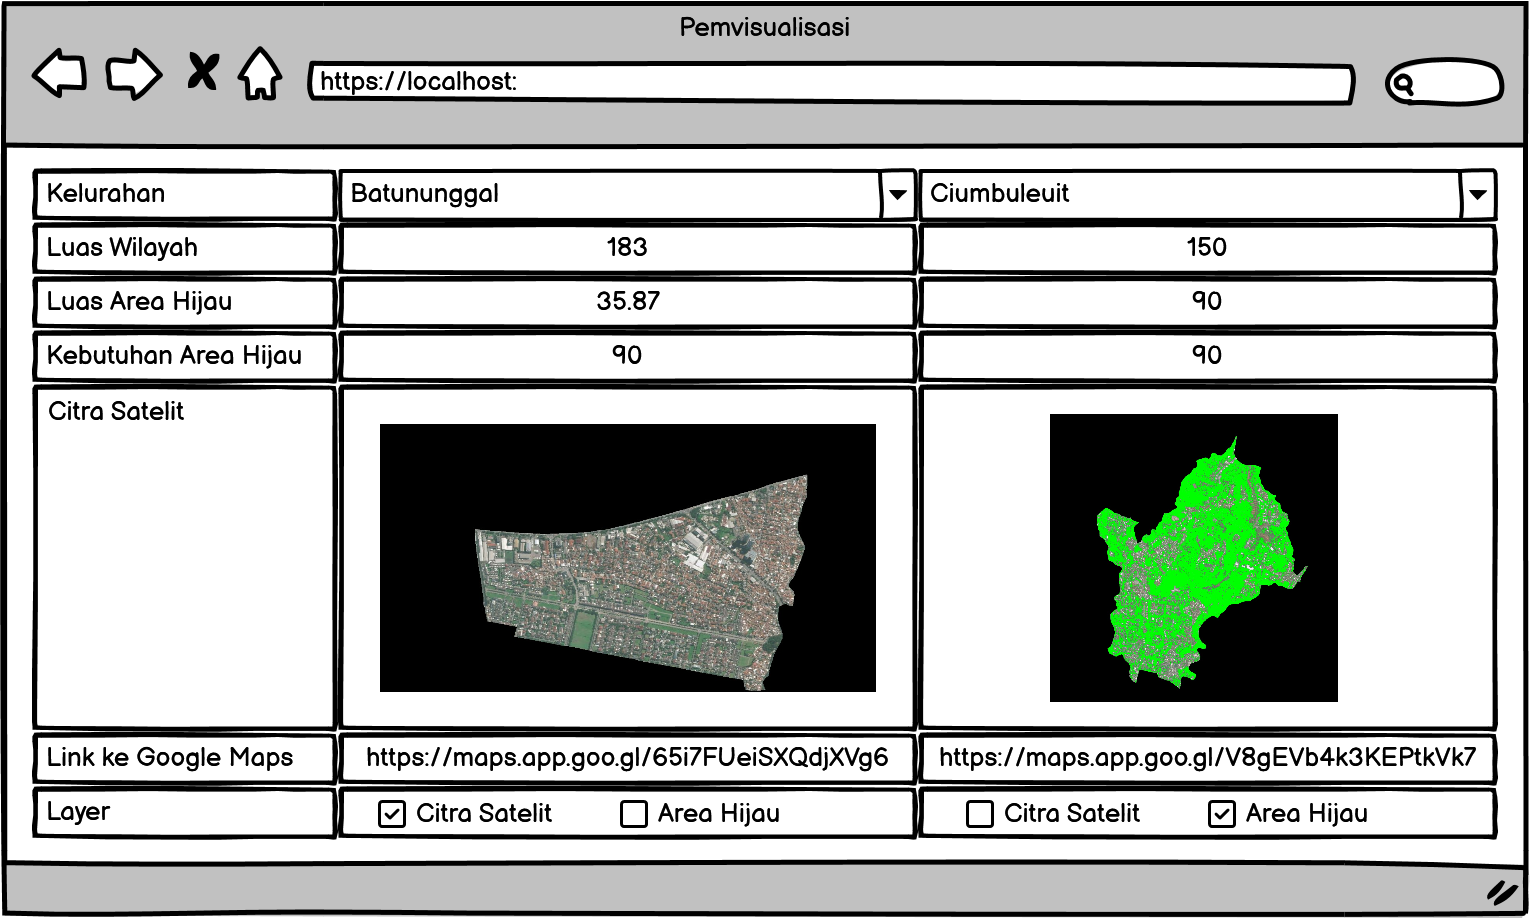
\includegraphics[width=0.8\textwidth]{Gambar/perancangan.png}
	\caption{Rancangan Antarmuka}
	\label{fig:rancanganAntarmuka}
\end{figure} 